% Isolation-contract figure for Ch18 ("Sub-Agents: The Context-Isolation Primitive").
% Standalone TikZ; compiled by `book-scaffold build-figures` via pdflatex -> pdftocairo -> SVG.
% Main conversation -> one prompt string (the only input channel) -> fresh sub-agent window that
% inherits nothing; its reads/tool-calls/dead-ends stay inside; only the final message returns.
% fork_session deliberately inverts the input side (carries parent context in); return unchanged.
\documentclass[tikz,border=4mm]{standalone}
\usepackage{tikz}
\usetikzlibrary{positioning, arrows.meta, calc}

\begin{document}
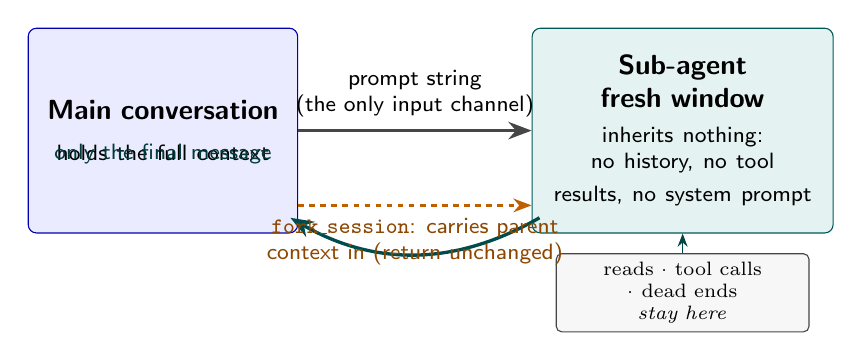
\begin{tikzpicture}[
  font=\sffamily,
  mainbox/.style={draw=blue!70!black, fill=blue!8, rounded corners=3pt, align=center,
    text width=3.0cm, minimum height=2.6cm, inner sep=6pt},
  subbox/.style={draw=teal!70!black, fill=teal!10, rounded corners=3pt, align=center,
    text width=3.4cm, minimum height=2.6cm, inner sep=6pt},
  inner/.style={draw=gray!55!black, fill=gray!6, rounded corners=2pt, align=center,
    text width=3.0cm, inner sep=3pt, font=\scriptsize},
  chan/.style={-Stealth, very thick, draw=gray!55!black},
  ret/.style={-Stealth, very thick, draw=teal!60!black},
  forkarr/.style={-Stealth, thick, draw=orange!75!black, dash pattern=on 2pt off 2pt}
]

\node[mainbox] (main) at (0,0)
  {{\bfseries Main conversation}\\[3pt]\footnotesize holds the full context};

\node[subbox] (sub) at (6.6,0)
  {{\bfseries Sub-agent}\\{\bfseries fresh window}\\[3pt]\footnotesize inherits nothing:\\no history, no tool\\results, no system prompt};

% the only input channel
\draw[chan] (main.east) -- (sub.west)
  node[midway, above=1pt, font=\sffamily\footnotesize, align=center] {prompt string\\(the only input channel)};

% what stays inside the sub-agent
\node[inner, below=0.25cm of sub] (stays) {reads · tool calls · dead ends\\\emph{stay here}};
\draw[draw=teal!55!black, -Stealth] (stays.north) -- (sub.south);

% the return contract
\draw[ret] ($(sub.south west)+(0.1,0.2)$) to[out=210, in=-30] ($(main.south east)+(-0.1,0.2)$)
  node[midway, below=1pt, font=\sffamily\footnotesize, text=teal!45!black] {only the final message};

% fork_session inverts the input side
\draw[forkarr] ($(main.east)+(0,-0.95)$) -- ($(sub.west)+(0,-0.95)$)
  node[midway, below=1pt, font=\sffamily\footnotesize, text=orange!55!black, align=center]
  {\texttt{fork\_session}: carries parent\\context in (return unchanged)};

\end{tikzpicture}
\end{document}
